Для впевненості у вирішенні проблеми уточнення маски хмарності, було проведено дослідження
та зроблена оцінка точності. Для цього знову був взятий знімок (рис. \ref{fig:accuracy-region})
частини Київської області та побудовано власноруч реальну маску хмар.

\begin{figure}[H]
	\centering
	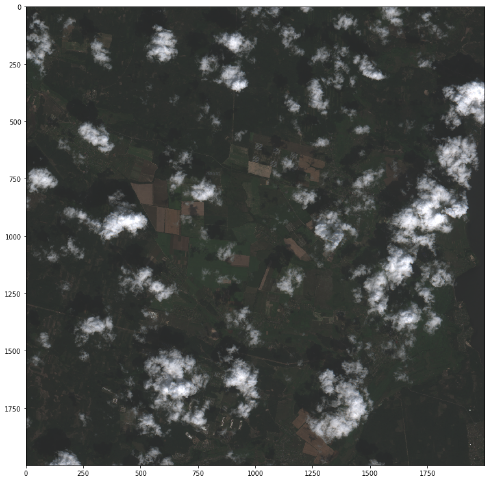
\includegraphics[width=0.4\textwidth]{images/image18}
	\caption{Область для оцінки точності \label{fig:accuracy-region} }
\end{figure}

Для демонстрації була взята маска верхнього лівого квадрата 500х500 (рис.\ref{fig:etalon-mask}).

\begin{figure}[H]
	\centering
	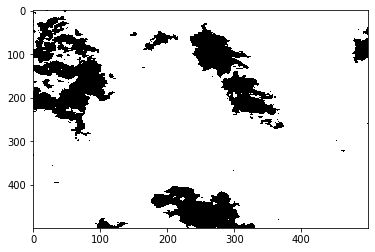
\includegraphics[width=0.5\textwidth]{images/image19}
	\caption{Еталонна маска \label{fig:etalon-mask} }
\end{figure}